\section{Vågutbredning på VHF, UHF, SHF och EHF}

\subsection{Allmänt}
Frekvensområdet 30--300000~MHz delas upp
i följande mindre avsnitt som kallas \\
VHF (Very High Frequency, 30--300~MHz), \\
UHF (Ultra High Frequency, 300--3000~MHz), \\
SHF (Super High Frequency, 3--30~GHz) och \\
EHF (Extra High Frequency, 30--300~GHz). \\

På VHF och högre frekvenser (tidigare UKV) förekommer sällan någon
vågutbredning via jonosfären annat än under tiden för maximal sol
aktivitet. I stället utnyttjas den lägre delen av atmosfären och
knappast högre än 4--5~km över jordytan. Denna del av atmosfären
kallas för troposfär och vågutbredningen därför för troposfärisk
vågutbredning.

All vågutbredning i troposfären förutsätter i princip optisk
sikt. Emellertid förekommer en viss vågavböjning utmed jordytan,
varför den praktiska räckvidden utmed siktlinjen är något längre än
till den optiska horisonten. Man talar om radiohorisont.

\emph{Brytningsindex} i atmosfären är en viktig faktor för
vågutbredning bortom frisiktsavståndet, speciellt vid frekvenser över
100~MHz. Även den splittring av vågorna som uppstår när de träffar
oregelbundenheter i atmosfären kan utnyttjas för kommunikation på
avstånd som är flera gången frisiktsavståndet

Vid högre frekvenser begränsas emellertid räckvidden av atmosfärens
dämpande inverkan. Likaså förloras vågenergi i den topografi,
vegetation och bebyggelse som ligger i siktlinjen mellan sändare och
mottagare. I gynnsamma fall är det dock möjligt att överbrygga avstånd
på upp till 1000~km genom troposfären. Sådana avstånd kallas för
överräckvidd.

\subsection{Troposfären -- Troposcatter}
\textbf{
HAREC a.\ref{HAREC.a.7.10}\label{myHAREC.a.7.10}
}

När en kallfront nära jordytan stöter samman med en varmfront
uppstår turbulens i luften med elektriska uppladdningar i
gränsskiktet som följd.

Under sådana väderförhållanden kan radiovågor i VHF-området och
däröver att brytas eller splittras upp när de träffar det laddade
gränsskiktet -- troposcatter. Då kan oväntade radiokontakter uppnås.

\subsection{Temperaturinversion}
\textbf{
HAREC a.\ref{HAREC.a.7.12}\label{myHAREC.a.7.12}
}

När ett varmt luftskikt lägger sig över ett kallare luftskikt uppstår
en s.k. temperaturinversion.

Vågor på VHF och UHF bryts då mot gränsskiktet och böjs av mot
jordytan. Om det finns två inversionsskikt samtidigt, så kan de bilda
en slags vågledare, s.k. dukt (eng. duct = ledning). En räckvidd på
600--1300~km kan uppnås. Denna typ av vågutbredning förekommer ofta
vid högt atmosfärstryck under sommaren.

\subsection{Reflexion mot \(\mathrm{E_s}\) (sporadiskt E)}
\textbf{
HAREC a.\ref{HAREC.a.7.13}\label{myHAREC.a.7.13}
}

Vid stark solinstrålning bildas, på de lägre latituderna, joniserade
gasmoln på en höjd av ca 120~km och med en oregelbunden fördelning.

Den kritiska frekvensen är hög för \(\mathrm{E_s}\)-skiktet och det
kan även reflektera vågor på VHF och UHF så effektivt att avstånd av
1000--4000~km kan överbryggas.

\subsection{Aurora-reflexion}
\textbf{
HAREC a.\ref{HAREC.a.7.14}\label{myHAREC.a.7.14}
}

Soleruptioner -- flares -- utstrålar stora mängder ultraviolett ljus och
kastar ut elektriskt laddade partiklar, som efter 1--2 dagar fångas upp
av jordens magnetosfär och tränger ner i polarzonerna. När partiklarna
kolliderar med atmosfären bildas det polarsken i form av lysande
''draperier'' -- Aurora (kallat norrsken på norra halvklotet) -- samtidigt
som atmosfären joniseras. Aurora är joniserade skikt i samma plan som
jordens magnetfält och speciellt vågor med frekvenser över 30~MHz
reflekteras emot dessa.

VHF- och UHF-kommunikation kan ske med hjälp av aurorareflexion. De
signaler som reflekteras av Aurora är kraftigt distorderade och har
förlorat all ton. Den reflekterade signalen blir bred i frekvens,
vilket emellertid gynnar kommunikation med telegrafi när signalerna är
svaga. Oftast är endast telegrafiförbindelser i långsam takt möjliga.
Vid starkare Aurora går också SSB att använda.

\subsection{Reflexion mot meteorer -- Meteorscatter}
\textbf{
HAREC a.\ref{HAREC.a.7.15}\label{myHAREC.a.7.15}
}

Radiovågor på VHF och UHF reflekteras mot joniserade spår efter det
meteorgrus som faller in i jordatmosfären. Detta fenomen kan utnyttjas
för radioförbindelser.

Joniseringen sker när partiklarna passerar genom E-skiktet och brinner upp.
Eftersom joniseringen har en varaktighet av endast 0,1--10~sekunder måste
\emph{MS-förbindelser} planeras och förberedas väl.
Förbindelserna begränsas vanligen till utbyte av anropssignaler och
signalrapporter med höghastighetstelegrafi med en hastighet av
300--3000~tecken per minut.
Under de större meteorskurarna kan kontakter uppnås utan överenskommelser på
förhand (skeds), både på telegrafi (CW) och telefoni (SSB).

\subsection{EME-förbindelser}
\textbf{
HAREC a.\ref{HAREC.a.7.16}\label{myHAREC.a.7.16}
}

Radioförbindelse från en punkt på jorden till en annan kan åstadkommas
genom reflexion av VHF-/UHF-signaler mot månen. EME-förbindelser
(Earth-Moon-Earth) kallas även Moon Bounce. EME-förbindelser kräver
antenner med mycket hög riktverkan, mycket hög sändareffekt och
känsliga mottagare.

\subsection{Markbaserade relästationer}

\begin{figure}
  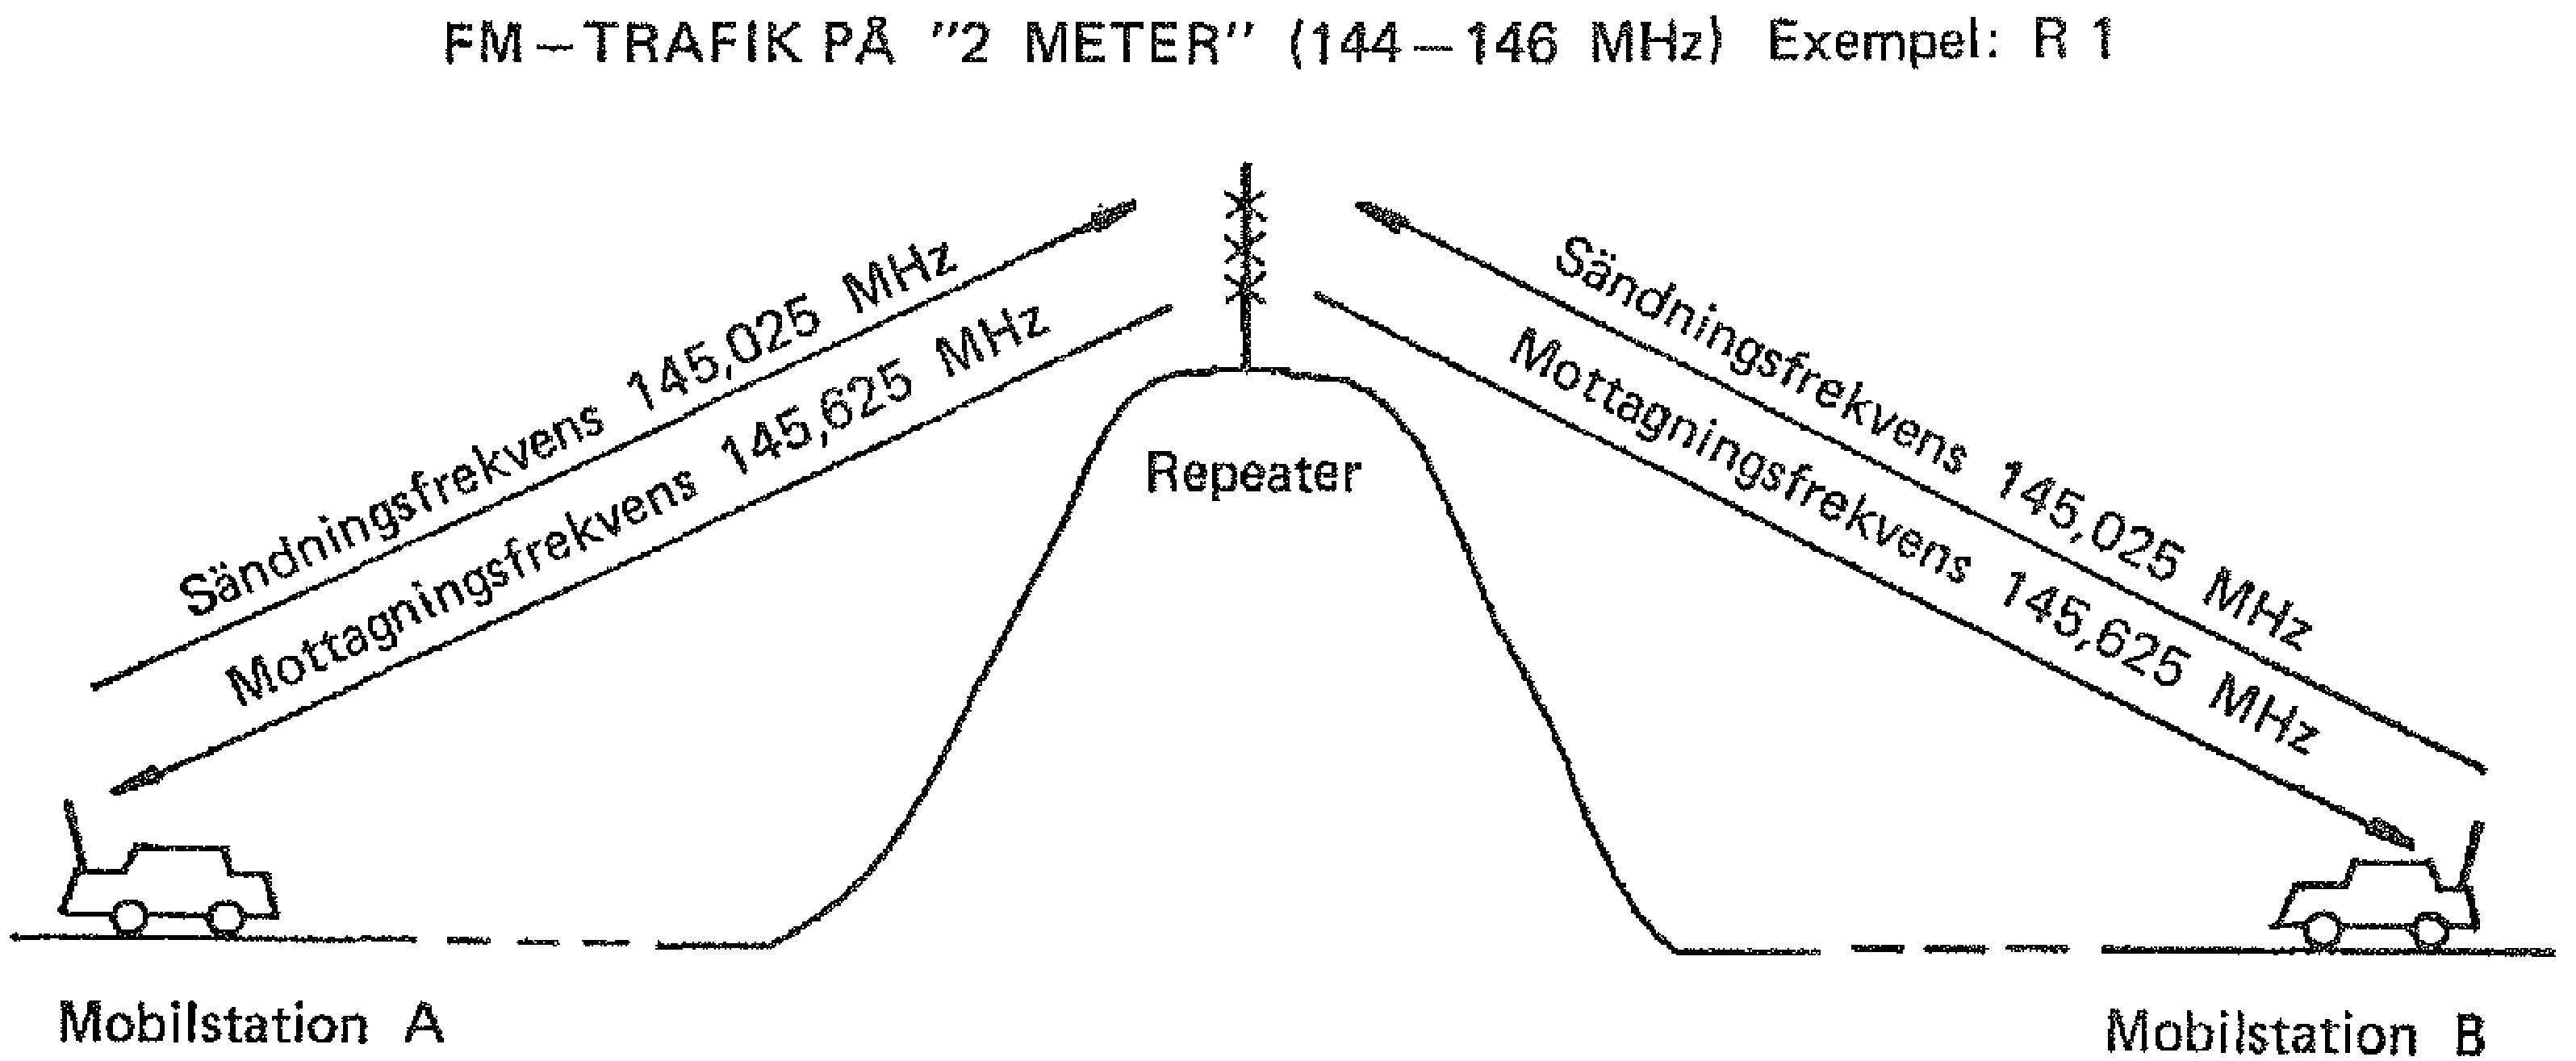
\includegraphics[width=\textwidth]{images/cropped_pdfs/bild_2_7-12.pdf}
  \caption{Markbaserad repeater}
  \label{fig:bildII7-12}
\end{figure}

På VHF och högre frekvenser kan man, som tidigare beskrivits, endast
uppnå radiokontakter hitom den s.k. radiohorisonten.

\hilight{TODO: Beskriv undantagen från detta - Es, tropo, meteorscatter, m.m.}

För att överbrygga detta hinder används relästationer, se bild
\ref{fig:bildII7-12}. Den slags
relästation, som allmänt kallas repeater, tar emot det den hör på en
viss fast frekvens och återutsänder detta på en viss annan fast
frekvens. Se bandplan i appendix \ref{svenska bandplaner}.

\subsection{Rymdsatellit-baserade relästationer}

Radiovågor med tillräckligt hög frekvens kan passera genom
jonosfärskikten. Detta möjliggör radioförbindelser VHF/UHF/SHF mellan
stationer på jorden med hjälp av relästationer i rymdsatelliter.

För amatörradiotrafik över rymdsatelliter används vanligen den slags
relästation, som kallas \emph{transponder}. En sådan tar emot allt det
den hör inom ett helt frekvensband och återutsänder detta i ett helt
annat frekvensband. På så sätt kan trafik över satellit ske på ett
jämförbart sätt som vid direktkontakt mellan jordbaserade stationer.

Satellitbaserade linjärtranspondrar med amatörradioutrustning finns i
OSCAR-satelliterna (OSCAR = Orbiting Satellite Carrying Amateur
Radio). Dessa har konstruerats och byggts av amatörradiogrupper.

OSCAR-satelliterna har många olika transpondrar i funktion, vilka var
och en arbetar med olika kombinationer av sändningsslag (moder) och
frekvensband. Detta kallas numera att de har olika konfiguration.

En vanlig konfiguration av transponder är CONFIG-V/U (f.d. MOD-J) där
upplänken är på VHF-bandet, t ex. 145,900--146,000~MHz och nerlänken på
UHF-bandet t.ex.  435,800--435,900~MHz. Varje upplänk-frekvens
motsvarar en bestämd nerlänk-frekvens, t.ex. upp 145,950 och ner
435,850~MHz. Trafiken övertranspondern kan därför ske i full duplex.

Man kan då prata och lyssa samtidigt i båda riktningarna, vilket
starkt förbättrar trafiken och gör samtalen roligare och
intressantare.

En s.k. linjär transponder kan inte bara överföra FM, utan även SSB,
tontelegrafi och SSTV. Dessutom även RTTY och andra digitala
trafiksätt.

Nästan alla amatörradioband med tillräckligt hög frekvens används i
olika kombinationer som upp- och nerlänkar i de olika
OSCAR-satelliterna. AMSAT är den organisation, som fortlöpande
informerar om amatörradiosatelliter.

\hilight{TODO: info om AMSAT-SM}

\begin{figure}
  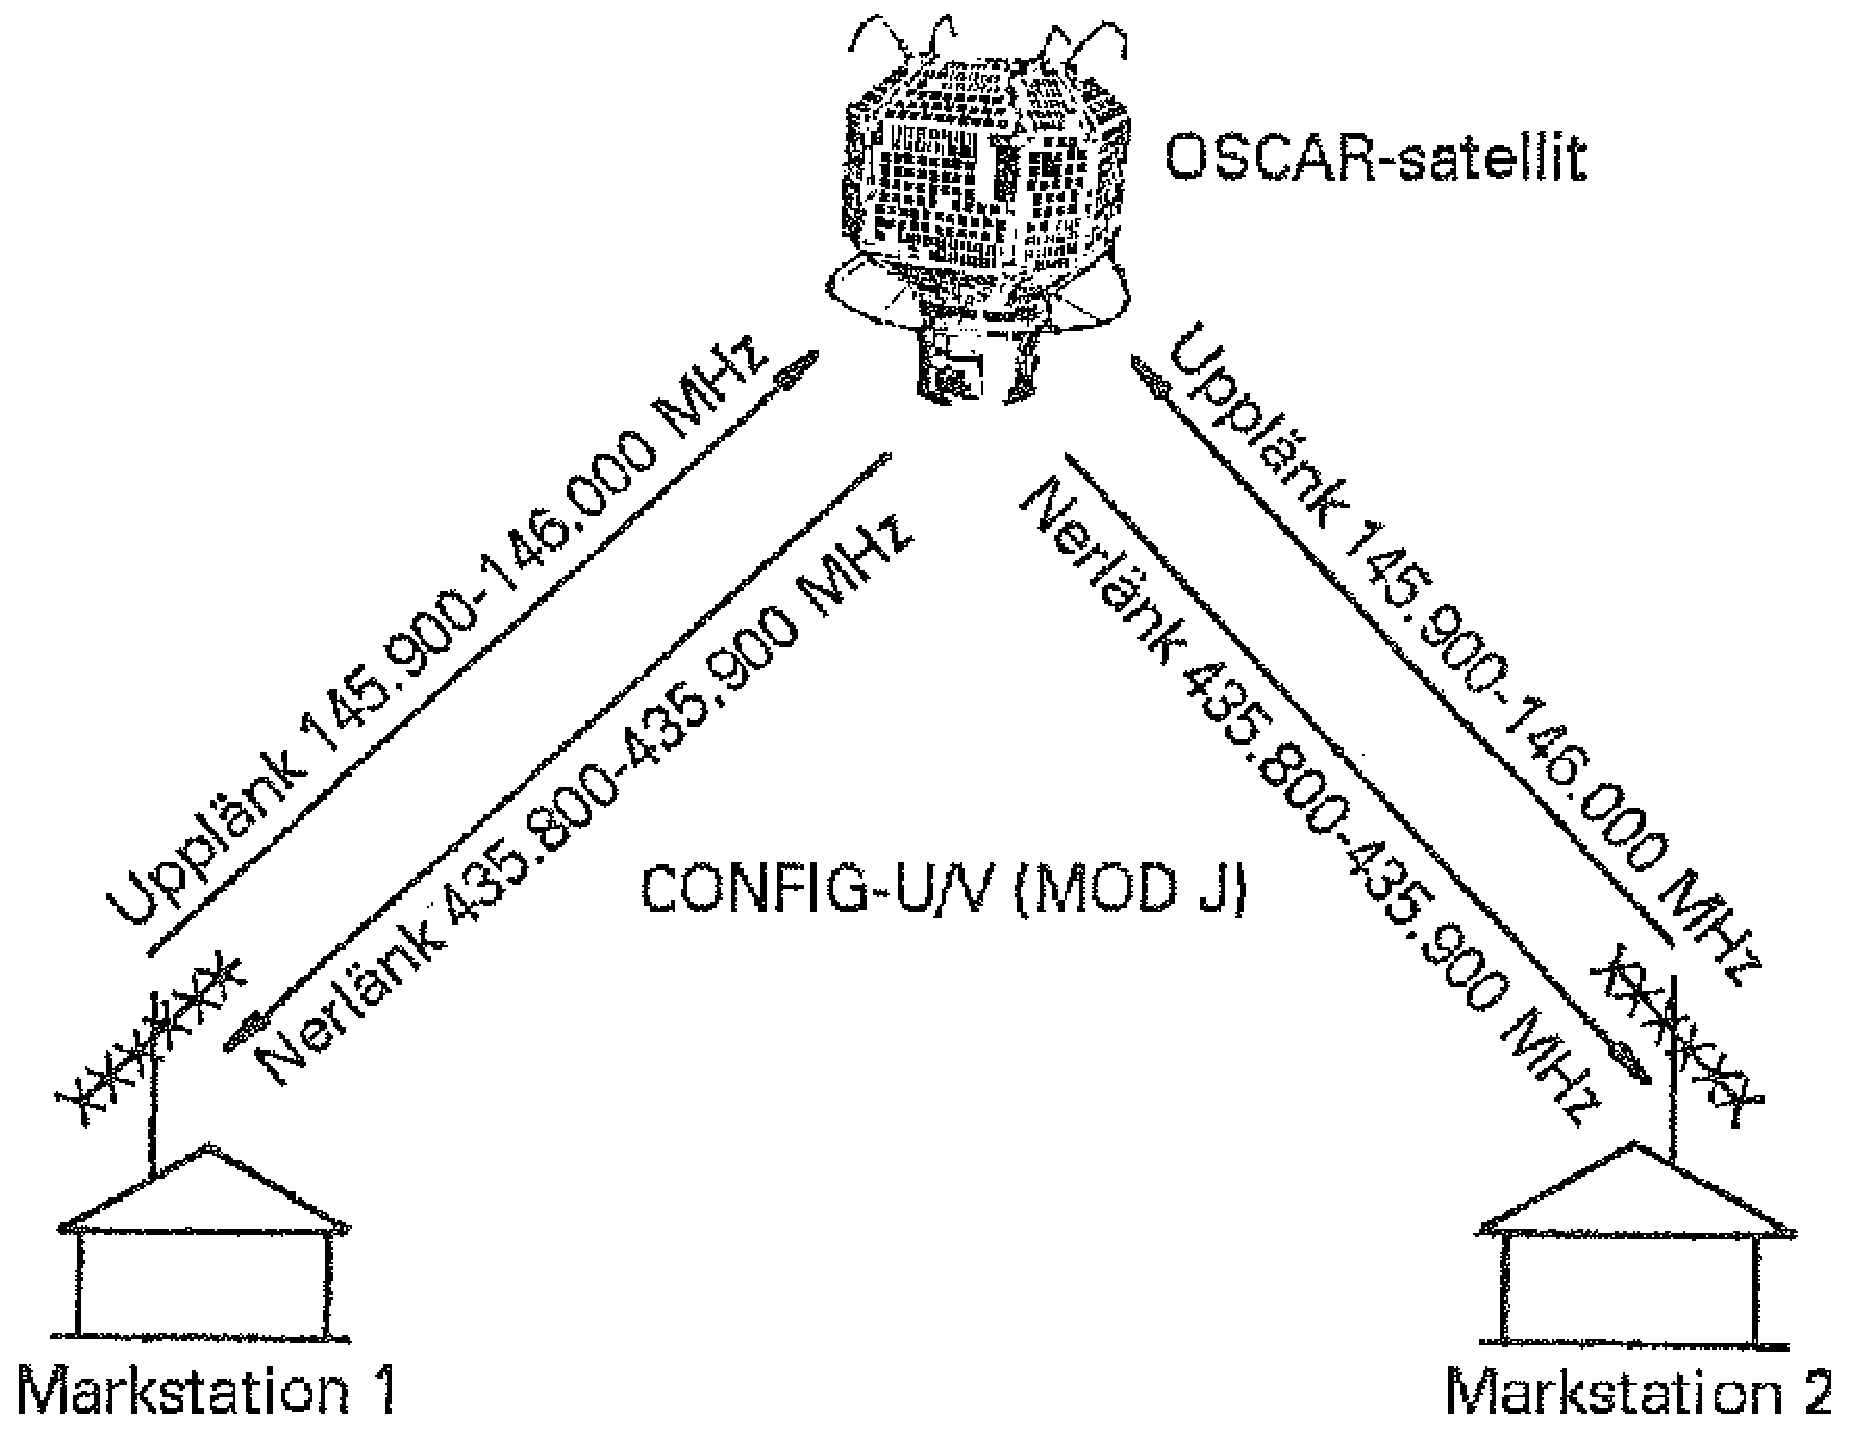
\includegraphics[width=\textwidth]{images/cropped_pdfs/bild_2_7-13.pdf}
  \caption{Transponder i rymdsatellit}
  \label{fig:bildII7-13}
\end{figure}

Amatörradion utvecklas mycket snabbt genom den satellitbaserade
verksamheten och det kommer upp allt mer sofistikerade
OSCAR-satelliter. Tendensen är att man efter hand går över till allt
högre frekvensband och allt mera av digitala sändningsslag.

Med hjälp av satellit kan förbindelseavståndet bli mycket stort även
med enkel utrustning och små antenner. En fördel med kommunikation
över rymdsatellit är också att den till största delen är oberoende av
vågutbredningsvillkoren.

Se bild \ref{fig:bildII7-13}.
